\documentclass[iop, twocolappendix, numberedappendix, tighten, appendixfloats]{emulateapj}
\citestyle{apj}

\usepackage[stable]{footmisc}
\usepackage{graphicx}
\usepackage{hyperref}
\usepackage{txfonts}
%\usepackage{hyperref}
\usepackage{natbib}
\bibpunct[, ]{(}{)}{;}{a}{}{,}
%\bibliographystyle{./bibtex/apj}

\newcommand{\farc}{\hbox{$.\!\!^{\prime\prime}$}} 
\newcommand{\ergA}{$\rm{erg\,cm^{-2}\,s^{-1}\,\AA^{-1}}$} 
\newcommand{\erg}{$\rm{erg\,cm^{-2}\,s^{-1}}$} 
\newcommand{\kms}{$\rm{km\,s^{-1}}\,$}

\newcommand{\griz}{$g' r' i' z'$}
\newcommand{\JHK}{$JHK_{\rm{s}}$}
\newcommand{\gK}{$g' r' i' z' JHK_{\rm{s}}$}
\newcommand{\Msun}{$M_\odot$}
\newcommand{\lya}{Ly$\alpha$} 
\newcommand{\lyb}{Ly$\beta$} 
\newcommand{\hb}{H$\beta$} 
\newcommand{\ha}{H$\alpha$} 
\newcommand{\oi}{[\ion{O}{1}]} 
\newcommand{\sii}{[\ion{S}{2}]} 
\newcommand{\oii}{[\ion{O}{2}]$\lambda$3727} 
\newcommand{\oiii}{[\ion{O}{3}]$\lambda$5007}
\newcommand{\nii}{[\ion{N}{2}]} 
\newcommand{\feii}{\ion{Fe}{2}} 
\newcommand{\civ}{\ion{C}{4}} 
\newcommand{\cii}{\ion{C}{2}}
\newcommand{\mgii}{\ion{Mg}{2}} 
\newcommand{\hi}{\ion{H}{1}} 
\newcommand{\ali}{\ion{Al}{1}} 
\newcommand{\SIii}{\ion{Si}{2}} 
\begin{document}
	
	\title{\vspace{-0.5cm}The X-shooter GTO sample of GRB afterglow and host Galaxy spectra}
	\altaffiltext{$^{\dag}$}{Based on observations collected at the European Southern Observatory, Paranal, 
		Chile, Program ID: 084.A-0260, 085.A-009, 086.A-0073, 087.A-0055.}
	
	\author{
		J.~Selsing\altaffilmark{1}, 
		D.~Malesani\altaffilmark{1}, 
		P.~Goldoni\altaffilmark{14}, 
		T.~Kr\"{u}hler\altaffilmark{1}, 
		J.~P.~U. Fynbo\altaffilmark{1}, 
		A.~de~Ugarte~Postigo\altaffilmark{11}, 
		J.~Japelj\altaffilmark{20},
		P.~D'Avanzo,
		Z.~Cano,
		S.~Covino\altaffilmark{10}, 
		V.~D'Elia\altaffilmark{7, 12}, 
		H.~Flores,
		O.~E.~Hartoog\altaffilmark{6},
		J.~Hjorth\altaffilmark{1}, 
		P.~Jakobsson\altaffilmark{5}, 
		A.~Levan,
		A.~Melandri,
		S.~Piranomonte \altaffilmark{7},
		R.~S\'anchez-Ram\'irez\altaffilmark{11},
		S.~Schulze\altaffilmark{17, 18}, 
		N.~R.~Tanvir\altaffilmark{19},
		C.~Th{\"o}ne,
		S.~D.~Vergani\altaffilmark{7, 8},
		P.~M.~Vreeswijk\altaffilmark{3}, 
		D.~J.~Watson\altaffilmark{1},
		K.~Wiersema\altaffilmark{19},
		D.~Xu\altaffilmark{1}
		L.~Christensen\altaffilmark{1},
		A.~De~Cia\altaffilmark{3}, 
		L.~Kaper\altaffilmark{6}, 
		L.~A.~Antonelli,
		F.~Fiore,
		A.~Gomboc,
		P.~Groot,
		F.~Hammer,
		C.~Ledoux\altaffilmark{2}, 
		E.~Maiorano,
		B.~Milvang-Jensen\altaffilmark{1}, 
		E.~Palazzi,
		E.~Pian,
		J.~Schaye,
		G.~Tagliaferri\altaffilmark{7},
		R.~A.~M.~J.~Wijers\altaffilmark{6}
	}
	
	\altaffiltext{1}{Dark Cosmology Centre, Niels Bohr Institute, University of Copenhagen, Juliane Maries Vej 30, 2100 K\o benhavn \O, Denmark}
	\altaffiltext{2}{European Southern Observatory, Alonso de C\'{o}rdova 3107, Vitacura, Casilla 19001, Santiago 19, Chile}
	\altaffiltext{3}{Department of Particle Physics and Astrophysics, Faculty of Physics, Weizmann Institute of Science, Rehovot 76100, Israel}
	\altaffiltext{4}{Th\"uringer Landessternwarte Tautenburg, Sternwarte 5, 07778 Tautenburg, Germany}
	\altaffiltext{5}{Centre for Astrophysics and Cosmology, Science Institute, University of Iceland, Dunhagi 5, IS-107 Reykjavik, Iceland}
	\altaffiltext{6}{Astronomical Institute Anton Pannekoek, University of Amsterdam, Science Park 904, NL-1098 XH Amsterdam, the Netherlands}
	\altaffiltext{7}{INAF-Osservatorio Astronomico di Roma, Via Frascati 33, I-00040 Monteporzio Catone, Italy}
	\altaffiltext{8}{GEPI-Observatoire de Paris, CNRS UMR 8111, Univ. Paris-Diderot, 5 Place Jules Janssen - 92190 Meudon, France}
	\altaffiltext{9}{American River College, Physics and Astronomy Dpt., 4700 College Oak Drive, Sacramento, CA 95841, USA}
	\altaffiltext{10}{INAF, Osservatorio Astronomico di Brera, Via E. Bianchi 46, I-23807 Merate, Italy}
	\altaffiltext{11}{Instituto de Astrof\'{\i}sica de Andaluc\'{\i}a (IAA-CSIC), Glorieta de la Astronom\'{\i}a s/n, 18008, Granada, Spain}
	\altaffiltext{12}{ASI-Science Data Centre, Via Galileo Galilei, I-00044 Frascati, Italy}
	\altaffiltext{13}{Institute of Experimental and Applied Physics, Czech Technical University in Prague, Horska 3a/22, 128 00 Prague 2, Czech Republic}
	\altaffiltext{14}{APC, Astroparticules et Cosmologie, Universite Paris Diderot, CNRS/
		IN2P3, CEA/Irfu, Observatoire de Paris, Sorbonne Paris Cite, 10, Rue Alice Domon et L
		eonie Duquet, 75205 Paris Cedex 13, France}
	\altaffiltext{15}{Max-Planck-Institut f\"{u}r extraterrestrische Physik, Giessenbachs
		tra\ss e, 85748 Garching, Germany}
	\altaffiltext{16}{Universit\`a degli studi di Milano-Bicocca, Piazza della Scienza 3,
		20126, Milano, Italy}
	\altaffiltext{17}{Pontificia Universidad Cat\'{o}lica de Chile, Departamento de Astro
		nom\'{\i}a y Astrof\'{\i}sica, Casilla 306, Santiago 22, Chile}
	\altaffiltext{18}{Millennium Center for Supernova Science}
	\altaffiltext{19}{Department of Physics and Astronomy, University ofLeicester, University Road, Leicester, LE1 7RH, UK}
	\altaffiltext{20}{University of Ljubljana,Department of Physics,Faculty of Mathematics \& Physics,SI}\
	
	\begin{abstract}
		Later
	\end{abstract}
	
	\keywords{Gamma-ray burst: individual: GRB~120815A --- galaxies: high-redshift --- ISM: molecules --- dust, extinction }
	
	\section{Introduction}
	
	\section{Observations}
	
	\LongTables
	
	\begin{deluxetable*}{@{\extracolsep{\fill}}lcccccclc@{}}
		%\tabletypesize{\scriptsize}
		%\rotate
		\tablecaption{The full sample of afterglows or hosts observed in the program.
			We here list the burst names and details of the spectroscopic observations. The
			exposure times and slit widths are given in the order UVB/VIS/NIR. The column
			$\Delta t$ shows the time after trigger when the spectroscopic observation was
			started. Mag$_\mathrm{acq}$ gives the approximate magnitude (typically in the
			$R$-band) of the afterglow in the acquisition image.
			\label{sample}}
		\tablewidth{0pt}
		\tablehead{
			\colhead{GRB} &  \colhead{Exptime} & \colhead{Slit width} & \colhead{Airmass} & \colhead{Seeing} & \colhead{$\Delta t$} & \colhead{Mag$_\mathrm{acq}$} & \colhead{Redshift} & \colhead{Ref}\\
			&  \colhead{(ks)}   & \colhead{(arcsec)} &   & \colhead{(arcsec)} & \colhead{(hr)}       &  & &  \\
		}
		\startdata
		GRB090313$^1$ 		& 6.9/6.9/6.9     	& 1.0/0.9/0.9 		& 1.2--1.4  	& 1.0  	&    45  	&  21.6  	& 3.3736 		& (1) \\
		GRB090530$^1$ 		& 4.8/4.8/4.8     	& 1.0/1.2/1.2 		& 1.6--2.2  	& 1.5  	&    20  	&  22    	& 1.266 		& (2) \\
		GRB090809$^1$ 		& 7.2/7.2/7.2     	& 1.0/0.9/0.9 		& 1.2--1.1  	& 0.9  	&  10.2  	&  21    	& 2.737  		& (2,3) \\
		GRB090926$^1$ 		& 7.2/7.2/7.2     	& 1.0/0.9/0.9 		& 1.4--1.5  	& 0.9  	&    22  	&  17.9  	& 2.1062 		& (4) \\
		GRB091018     		& 2.4/2.4/2.4     	& 1.0/0.9/0.9 		& 2.1--1.8  	& 0.8  	&   3.5  	&  19.1  	& 0.9710 		& (5) \\  
		GRB091127     		& 6.0/6.0/6.0     	& 1.0/0.9/0.9 		& 1.1--1.2  	& 1.0  	&   101  	&  21.2  	& 0.490  		& (6) \\
		GRB100205A     		& 10.8/10.8/10.8 	& 1.0/0.9/0.9 		& 1.9--1.8  	& 1.0  	&    71  	&   --   	&  --    		& (2) \\
		GRB100219A     		&  4.8/4.8/4.8   	& 1.0/0.9/0.9 		& 1.3--1.1  	& 0.7  	&  12.5  	&   23   	& 4.667  		& (7) \\
		GRB100316B     		&  2.4/2.4/2.4   	& 1.0/0.9/0.9 		& 2.0--2.4  	& 0.7  	&   0.7  	&  18.2  	& 1.18   		& (2) \\
		GRB100316D-1$^2$ 	&  7.2/7.2/7.2   	& 1.0/0.9/0.9 		& 1.2--1.5  	& 1.0  	&  12  		&   --   	& 0.059  		& (8) \\
		GRB100316D-2   		&  2.4/2.4/2.4   	& 1.0/0.9/0.9 		& 1.2--1.2  	& 1.0  	&    58  	&   --   	& 0.059  		& (8) \\
		GRB100316D-3   		&  2.4/2.4/2.4   	& 1.0/0.9/0.9 		& 1.2--1.2  	& 0.8  	&   192  	&   --   	& 0.059  		& (8) \\
		GRB100418A-1   		&  4.8/4.8/4.8   	& 1.0/0.9/0.9 		& 1.6--1.3  	& 0.7  	&   8.4  	&  18.1  	& 0.6235 		& (9) \\
		GRB100418A-2   		&  4.8/4.8/4.8   	& 1.0/0.9/0.9 		& 1.2--1.3  	& 0.6  	&    34  	&  19.2   	& 0.6235 		& (9) \\
		GRB100418A-3   		&  4.8/4.8/4.8   	& 1.0/0.9/0.9 		& 1.2--1.4  	& 0.7  	&    58  	&   --   	& 0.6235 		& (9) \\
		GRB100424A$^3$ 		&  4.8/4.8/4.8   	& 1.0/0.9/0.9 		& 1.1--1.2  	& 0.8  	&   --   	&   --   	& 2.465  		& (2) \\
		GRB100425A     		&  2.4/2.4/2.4   	& 1.0/0.9/0.9 		& 1.5--1.3  	& 0.7  	&   4.0  	&  20.6  	& 1.755  		& (2,3) \\
		GRB100621A     		&  2.4/2.4/2.4   	& 1.0/0.9/0.9 		& 1.3--1.4  	& 1.0  	&   7.1  	&   --   	& 0.542  		& (2) \\
		GRB100625A$^3$ 		&  4.8/4.8/4.8   	& 1.0/0.9/0.9 		& 1.1--1.0  	& 0.8  	&    13  	&   --   	& 0.452  		& (2) \\
		GRB100724A$^4$ 		&  4.2/4.2/4.2   	& 1.0/0.9/0.9 		& 1.5--2.3  	& 0.7  	&   0.2  	&   --   	& 1.288  		& (2) \\
		GRB100728B$^5$ 		&  7.2/7.2/7.2   	& 1.0/0.9/0.9 		& 1.5--1.1  	& 0.5  	&    22  	&   23   	& 2.106  		& (2) \\
		GRB100814A-1$^4$ 	& 0.9/0.9/0.9  		& 1.0/0.9/0.9 		& 1.9--1.7  	& 0.5  	&   0.8  	&   19   	& 1.44   		& (2) \\
		GRB100814A-2   		&  4.8/4.8/4.8   	& 1.0/0.9/0.9 		& 1.5--1.2  	& 0.6  	&   1.4  	&   19   	& 1.44   		& (2) \\
		GRB100814A-3   		&  4.8/4.8/4.8   	& 1.0/0.9/0.9 		& 1.2--1.0  	& 0.6  	&   99   	&   20   	& 1.44   		& (2) \\
		GRB100816A$^6$ 		&  4.8/4.8/4.8   	& 1.0/0.9/0.9 		& 1.8--1.6  	& 0.8  	&   3.7  	&   --   	& 0.806  		& (2) \\
		GRB100901A     		&  2.4/2.4/2.4   	& 1.0/0.9/0.9 		& 1.5--1.5  	& 1.8  	&   66   	&   --   	& 1.408  		& (10) \\
		GRB101219A     		&  7.2/7.2/7.2   	& 1.0/0.9/0.9 		& 1.1--1.7  	& 2.0  	&   3.7  	&   --   	& 0.718  		& (2) \\
		GRB101219B-1   		&  4.8/4.8/4.8   	& 1.0/0.9/0.9 		& 1.6--2.6  	& 1.3  	&  11.6  	&   20   	& 0.5519 		& (11) \\
		GRB101219B-2   		&  7.2/7.2/7.2   	& 1.0/0.9/0.9 		& 1.2--2.0  	& 0.8  	&   394  	&  22.7  	& 0.5519 		& (11) \\
		GRB101219B-3   		&  7.2/7.2/7.2   	& 1.0/0.9/0.9 		& 1.4--2.1  	& 0.9  	&   886  	&   --   	& 0.5519 		& (11) \\
		GRB110128A     		&  7.2/7.2/7.2   	& 1.0/0.9/0.9 		& 2.0--1.6  	& 0.9  	&   5.5  	&  22.5  	& 2.339  		& (2) \\
		GRB110407A     		&  9.6/9.6/9.6   	& 1.0/0.9/0.9 		& 1.4--1.3  	& 2.0  	&  12.4  	&   23   	&  --    		& (2) \\
		GRB110709B$^1,3$ 	&  7.2/7.2/7.2 		& 1.0/0.9/0.9 		& 1.6--1.1  	& 1.0  	&   --   	&   --   	&  --    		& (2) \\
		GRB110715A     		&  0.6/0.6/0.6   	& 1.0/0.9/0.9 		& 1.1--1.1  	& 1.7  	&  12.3  	&  18.5  	& 0.82  		& (2) \\
		GRB%110721A     	&  2.4/2.4/2.4   	& 1.0/0.9/0.9 		& 1.2--1.4  	& 2.4  	&        	&        	& 0.382  		& (2) \\
		GRB110808A     		& 2.4/2.4/2.4    	& 1.0/0.9/0.9 		& 1.2--1.1  	& 1.1  	&   3.0  	&  21.2  	& 1.3488 		& (2) \\
		GRB110818A     		& 4.8/4.8/4.8    	& 1.0/0.9/0.9 		& 1.3--1.3  	& 1.0  	&   6.2  	&  22.3  	& 3.36   		& (2) \\
		GRB111005A$^3$ 		& 1.2/1.2/1.2    	& 1.0/0.9/0.9 		& 1.3--1.3  	& 0.7  	&   --   	&  --    	& 0.013? 		& (2) \\
		GRB111008A-1   		& 8.8/8.8/8.4    	& 1.0/0.9/0.9 		& 1.1--1.0  	& 1.2  	&   8.5  	&  21?   	& 4.9898 		& (12) \\
		GRB111008A-2   		& 8.0/8.0/7.2    	& 1.0/0.9/0.9 		& 1.3--1.0  	& 1.0  	&  20.1  	&  22?   	& 4.9898 		& (12) \\
		GRB111107A     		& 4.8/4.8/4.8    	& 1.0/0.9/0.9 		& 1.8--1.5  	& 0.7  	&   5.3  	&  21.5  	& 2.893  		& (2) \\
		GRB111117A$^6$ 		& 4.8/4.8/4.8    	& 1.0/0.9/0.9 		& 1.5--1.4  	& 0.6  	&    38  	&  --    	& 1.3?   		& (2) \\
		GRB111123A-1   		& 6.2/6.6/6.6    	& 1.0/0.9/0.9 		& 1.6--1.1  	& 1.0  	&  12.2  	&  $>$24 	& 3.1516 		& (2) \\
		GRB111123A-2$^3$ 	& 2.4/2.4/2.4  		& 1.0/0.9/0.9 		& 1.0--1.0  	& 0.5  	&   --   	&  --    	& 3.1516 		& (2) \\
		GRB111129A     		& 3.6/3.6/3.6    	& 1.0/0.9/0.9 		& 1.6--2.1  	& 1.7  	&        	&        	&  --    		& (2) \\
		GRB111209A-1   		& 4.8/4.8/4.8    	& 1.0/0.9/0.9 		& 1.1--1.2  	& 0.8  	&  17.7  	&  20.1  	& 0.677  		& (13) \\
		GRB111209A-2   		& 9.6/9.6/9.6    	& 1.0/0.9/0.9 		& 1.2--2.0  	& 0.8  	&  497   	&  23    	& 0.677  		& (13) \\
		GRB111211A$^1$ 		& 2.4/2.4/2.4    	& 1.0/0.9/0.9 		& 1.4--1.6  	& 0.6  	&   31   	&  19.5  	& 0.478  		& (2) \\
		GRB111228A     		& 2.4/2.4/2.4    	& 1.0/0.9/0.9 		& 1.4--1.4  	& 0.9  	&  15.9  	&  20.1  	& 0.716  		& (2) \\
		GRB120118B$^3$ 		& 3.6/3.6/3.6    	& 1.0/0.9/0.9 		& 1.1--1.0  	& 1.0  	&   --   	&  --    	& 2.943  		& (2) \\
		GRB120119A-1   		& 2.4/2.4/2.4    	& 1.0/0.9/0.9 		& 1.1--1.1  	& 0.6  	&   1.4  	&   17   	& 1.728  		& (2) \\
		GRB120119A-2   		& 1.2/1.2/1.2    	& 1.0/0.9/0.9 		& 1.8--1.9  	& 0.6  	&   4.5  	&   20   	& 1.728  		& (2) \\
		GRB120119A-3$^3$ 	& 4.8/4.8/4.8  		& 1.0/0.9/0.6JH 	& 1.0--1.1  	& 1.1 	&   --   	&   --   	& 1.728  		& (2) \\
		GRB120211      		&                	&             		&           	&      	&        	&         	& 2.346 		& (2) \\
		GRB120224A     		& 2.4/2.4/2.4    	& 1.0/0.9/0.9 		& 1.7--2.1  	& 1.4  	&  19.8  	&   22.3 	&  --    		& (2) \\
		GRB120311A     		& 2.4/2.4/2.4    	& 1.0/0.9/0.9 		& 1.6--1.4  	& 0.6  	&   3.7  	&   21.6 	&  --    		& (2) \\
		GRB120327A-1   		& 2.4/2.4/2.4    	& 1.0/0.9/0.9 		& 1.6--1.4  	& 0.5  	&   2.1  	&   18.8 	& 2.815  		& (14) \\
		GRB120327A-2   		& 4.2/4.2/4.2    	& 1.0/0.9/0.9 		& 1.0--1.1  	& 1.0  	&    29  	&   22.5 	& 2.815  		& (14) \\
		GRB120404A     		& 9.6/9.6/9.6    	& 1.0/0.9/0.9JH 	& 1.7--1.3 		& 1.3 	&  15.7  	&   21.3 	& 2.876  		& (2) \\
		GRB120422A-1   		& 4.8/4.8/4.8    	& 1.0/0.9/0.9 		& 1.3--1.3  	& 0.6  	&  17.2  	&   22.0 	& 0.283  		& (15) \\
		GRB120422A-2   		& 4.8/4.8/4.8    	& 1.0/0.9/0.9 		& 1.3--1.4  	& 0.9  	&  113   	&   --   	& 0.283  		& (15) \\
		GRB120422A-3   		& 4.8/4.8/4.8    	& 1.0/0.9/0.9 		& 1.4--1.7  	& 1.0  	&  210   	&   --   	& 0.283  		& (15) \\
		GRB120422A-4   		& 4.8/4.8/4.8    	& 1.0/0.9/0.9JH 	& 1.3--1.4 		& 0.6  	& 449   	&   --   	& 0.283  		& (15) \\
		GRB120422A-5   		& 4.8/4.8/4.8    	& 1.0/0.9/0.9JH 	& 1.3--1.6 		& 0.8  	& 593   	&   --   	& 0.283  		& (15) \\
		GRB120422A-6   		& 4.8/4.8/4.8    	& 1.0/0.9/0.9JH 	& 1.7--2.4 		& 2.5  	& 882   	&   --   	& 0.283  		& (15) \\
		GRB120422A-7   		& 4.8/4.8/4.8    	& 1.0/0.9/0.9JH 	& 1.5--1.9 		& 1.3  	& 906   	&   --   	& 0.283  		& (15) \\
		GRB120712A     		& 4.8/4.8/4.8    	& 1.0/0.9/0.9   	& 1.5--2.5 		& 1.3  	& 10.4  	&   21.5 	& 4.175  		& (2) \\
		GRB120714B     		& 4.8/4.8/4.8    	& 1.0/0.9/0.9JH 	& 1.5--1.2 		& 1.2  	&  7.8  	&   22.1 	& 0.398  		& (2)\\
		GRB120716A$^1$ 		& 3.6/3.6/3.6    	& 1.0/0.9/0.9JH 	& 1.8--2.6 		& 1.0  	&  62   	&   20.9 	& 2.486  		& (2) \\
		GRB120722A$^2$ 		& 4.8/4.8/4.8    	& 1.0/0.9/0.9   	& 1.3--1.3 		& 1.1  	& 10.3  	&   23.6 	& 0.959  		& (2) \\
		GRB120805A$^2$ 		& 3.6/3.6/3.6    	& 1.0/0.9/0.9JH 	& 1.3--1.7 		& 0.9  	& 218   	&   --   	& 2.8?   		& (2) \\
		GRB120815A     		& 2.4/2.4/2.4    	& 1.0/0.9/0.9   	& 1.3--1.4 		& 0.6  	&  1.7  	&   20   	& 2.358  		& (16) \\
		GRB120909A     		& 1.2/1.2/1.2    	& 1.0/0.9/0.9   	& 1.6--1.6 		& 1.4  	&  1.7  	&   21   	& 3.929  		& (2) \\
		GRB120923A     		& 9.6/9.6/9.6    	& 1.0/0.9/0.9JH 	& 1.2--1.4 		& 1.0  	& 18.5  	&   --   	& $\gtrsim8$ 	& (2) \\
		GRB121024A     		& 2.4/2.4/2.4    	& 1.0/0.9/0.9   	& 1.2--1.1 		& 0.6  	&  1.8  	&   20   	& 2.300  		& (17) \\
		GRB121027A     		& 8.4/8.4/8.4    	& 1.0/0.9/0.9   	& 1.3--1.3 		& 0.9  	&  69   	&  21.1  	& 1.773  		& (2) \\
		GRB121201A     		& 4.8/4.8/4.8    	& 1.0/0.9/0.9JH 	& 1.1--1.1 		& 0.9  	& 12.9  	&   23   	& 3.385  		& (2) \\
		GRB121229A     		& 4.8/4.8/4.8    	& 1.0/0.9/0.9JH 	& 1.4--1.2 		& 1.4  	&  2.0  	&  21.5  	& 2.707  		& (2) \\
		GRB130131B$^3$ 		& 7.2/7.2/7.2    	& 1.0/0.9/0.9JH 	& 1.3--1.6 		& 0.8  	&  --   	&   --   	& 2.539  		& (2) \\
		GRB130408A     		& 1.2/1.2/1.2    	& 1.0/0.9/0.9   	& 1.0--1.0 		& 1.0  	&  1.9  	&   20   	& 3.758  		& (2) \\
		GRB130418A     		& 1.2/1.2/1.2    	& 1.0/0.9/0.9   	& 1.4--1.3 		& 1.3  	&  4.6  	&   18.5 	& 1.218  		& (2) \\
		GRB130427A     		& 1.2/1.2/1.2    	& 1.0/0.9/0.9JH 	& 1.8--1.8 		& 0.8  	& 16.5  	&   19   	& 0.340  		& (18) \\
		GRB130427B     		& 1.2/1.2/1.2    	& 1.0/0.9/0.9JH 	& 1.2--1.0 		& 0.8  	& 20.3  	&   22.7 	& 2.78   		&  (2) \\
		GRB130603B$^6$ 		& 2.4/2.4/2.4    	& 1.0/0.9/0.9   	& 1.4--1.4 		& 1.1  	&  8.2  	&   21.5 	& 0.356  		& (19) \\
		GRB130606A     		& 4.2/4.2/4.2    	& 1.0/0.9/0.9JH 	& 1.7--1.9 		& 1.1  	&  7.1  	&   19   	& 5.91   		& (20) \\
		GRB130612A     		& 1.2/1.2/1.2    	& 1.0/0.9/0.9   	& 1.3--1.3 		& 1.4  	&  1.1  	&   21.5 	& 2.006  		& (2) \\
		GRB130615A     		& 1.2/1.2/1.2    	& 1.0/0.9/0.9   	& 2.1--2.2 		& 1.0  	&  0.8  	&   21   	& $~3$?  		& (2) \\
		GRB130701A     		& 1.2/1.2/1.2    	& 1.0/0.9/0.9JH 	& 2.0--2.0 		& 1.6  	&  5.5  	&   19.9 	& 1.155  		& (2) \\
		\enddata
		\tablenotetext{1}{Not part of the statistical sample}
		\tablenotetext{2}{Spectrum dominated by light from the host galaxy}
		\tablenotetext{3}{Spectrum of the host galaxy taken long after the burst}
		\tablenotetext{4}{RRM observation}
		\tablenotetext{5}{ADC malfunction during observation}
		\tablenotetext{6}{Short burst}
		\tablerefs{
			(1) \citet{DeUgartePostigo2010}; (2) This work ; (3) Skuladottir (2010);
			(4) \citet{DElia2010}; (5) \citet{Wiersema2012}; (6) \citet{Vergani2011, Cobb2010}; 
			(7) \citet{Thone2013}; (8) \citet{Bufano2012} ; (9) \citet{DeUgartePostigo2011} ;
			(10) \citet{Hartoog2013}; (11) \citet{Sparre2011}; (12) \citet{Sparre2014};
			(13) \citet{Levan2014}; (14) \citet{DElia2014}; (15) \citet{Schulze2014};
			(16) \citet{Kruhler2013}; (17} \citet{Friis2015}
	\end{deluxetable*}
	%-------------------------END TABLE---------------------------------------
	
	
	\subsection{RRM observations} \label{RRM}
	The rapid-response mode is 
	
	
	\section{Results}
	
	\subsection{Spectral resolution}
	The afterglow spectra described in this paper are obtained in
	Target-of-Opportunity (override) mode.
	In most cases there is therefore little possibility to tweak slit widths to the
	seeing at the time of observations (i.e. to optimise spectral resolution and
	signal to noise), and almost all our data is therefore taken with a fixed set
	of slit widths and binning, described above.
	In a fair number of cases, the seeing full width at half maximum (FWHM) is
	considerably smaller than the silt width, and the delivered spectral resolution
	will then be determined by the seeing rather than slit width, as afterglows are
	point sources (this is evidently not the case for extended sources, e.g for
	host galaxies).
	The delivered resolution for slit width dominated spectra post-reduction and
	extraction can easily be determined from the bright sky emission lines.
	For afterglow spectra with very high signal to noise, the delivered spectral
	resolution can at times be determined from the science data themselves.
	However, in the presence of multiple velocity components in absorption, other
	forms of line broadening, and a lack of lines at some redshifts, this is
	difficult to do at poorer signal to noise ratios (the majority of spectra in
	our sample).
	A broad starting value for the expect resolution will help fitting of these
	spectra, and can be important in upper limit determination, and for this reason
	we construct a aim to construct a crude relation between the seeing and the
	delivered resolution at our slit width, binning, and reduction pipeline
	settings.
	To this end we use observations of telluric standard stars that are taken with
	identical instrument settings as our afterglow spectra, usually just after the
	science data, as part of the ESO X-shooter calibration plan.
	These spectra have been reduced together with the afterglow spectra, using
	identical pipeline settings with the same version of the pipeline.
	First we fit a Gaussian function in the spatial direction of the trace of the
	standard star at 792 nm (i.e. in the VIS arm).
	After this, we fit a series of  20 telluric absorption lines in the telluric
	standard star spectra with Gaussians, taking care to select transitions that
	are not almost-resolved multiples, should be intrinsically unresolved, and are
	in areas with well defined continuum flux.
	We pick 34 telluric standard stars spanning a range of DIMM seeing values, with
	the majority between $0.5-1.5 arcsec$.
	The resulting distribution of spectral FWHM (km/s) as a function of spatial
	FWHM at 792 nm is fairly well described by a linear relation $a + b*x$, with
	$x$ the spatial FWHM in pixels (with 0.15 arc sec per pixel),  $a= 21.4 \pm
	1.3$ km/s, $b=1.4 \pm 0.2$.
	We use this linear relation as a way to estimate the spectral resolution for
	medium to poor signal to noise afterglow spectra in the VIS arm.
	To extend this to the UVB and NIR arm, we measured a series of lines in NIR arm
	spectra of a subset of 19 sources used for the VIS arm above, and find that the
	resulting distribution is consistent with a simple scaling of the VIS arm
	relation by the ratio of resolutions of the NIR and VIS arm for unresolved,
	slit filling, sources as given on the ESO instrument website.
	The UVB arm contains no suitable absorption lines to use, and we therefore use
	a scaled value as in the NIR arm.
	While this simple method is not terribly accurate (for one, the spatial profile
	of the trace is not a perfect Gaussian), but it gives a sufficiently accurate
	estimate for the analysis of these poor signal to noise science spectra.
	

%	\begin{figure}
%		%\vspace{11pc}   
%		%\includegraphics[width=10cm]{060218/6273fig1.ps}
%		\centerline{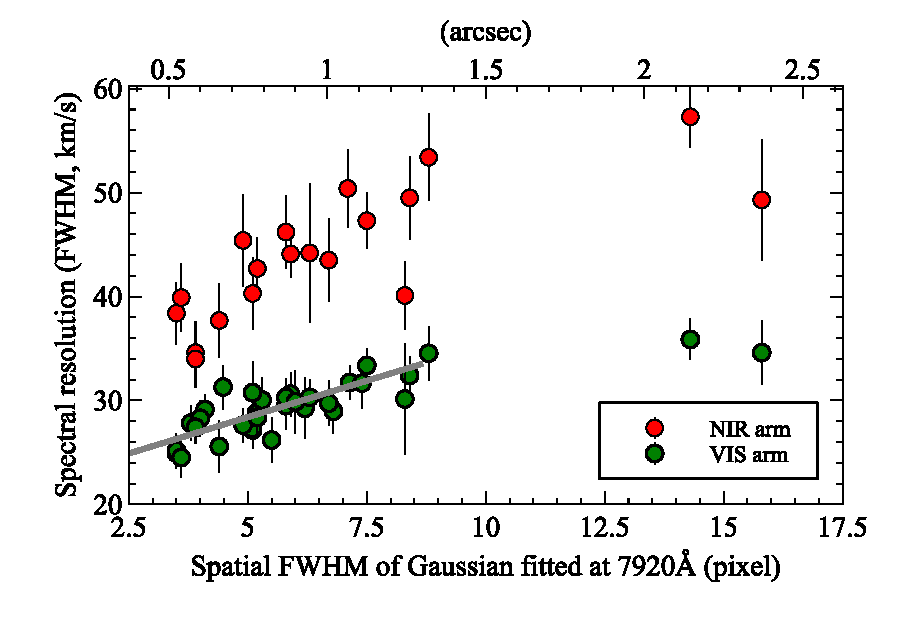
\includegraphics[width=8cm]{Resolution/resolution_paper.eps}}
%		\caption{Green datapoints show the FWHM (km/s) of Gaussian fits to unresolved telluric absorption lines in the VIS spectra, as a function of the FWHM of a Gaussian fit onto the trace in spatial direction at  792 nm. The lower horizontal axis is in units pixels, the top axis in arc seconds. The red datapoints show a subsample of NIR spectra.
%			The grey line shows a linear fit to the VIS datapoints. }
%		\label{fig:res}
%	\end{figure}
	
	\subsection{Correction for offsets in the wavelength calibration}    
	
	X-shooter, being installed at the VLT Cassegrain focusi is  prone to
	flexures during operations. The flexures modify the projection of the slit
	on the detector with respect to the one obtained in daytime calibration. 
	This require a modification of the wavelength solution in order to
	process correctly the night-time data. Part of this correction
	is performed by the pipeline using the frames taken
	during X-shooter Active Flexure Compensation procedure
	\footnote{X-shooter User Manual available at https://www.eso.org/sci/facilities/paranal/instruments/xshooter/doc.html}
	We corrected the remaining part using as a reference the sky
	emission lines present in the observed data.
	
	
	For every afterglow observation we reduced one frame individually in STARE mode without
	sky subtraction obtaining $\sim$ 100 sky spectra. The sky line list compiled at ESO for
	the E-ELT
	study\footnote{http://www.eso.org/sci/facilities/eelt/science/drm/tech\_data/data/optical\_ir\_sky\_lines.dat}
	from the work of (Hanuschik, 2003, A\&A, 407, 1157) and (Rousselot et al. (2000, A\&A, 354, 1134), was used as a reference.
	From this list, we selected a subset of bright and isolated lines. In the case of the OH doublets, unresolved at X-shooter resolution, we took as line position the average between the blue and red components. To find the offsets of the spectra, we fitted gaussians near the
	expected positions under IDL using the MPFIT software (Markwardt, 2009, Astronomical Society of the Pacific Conference Series, Vol. 411, ADASS XVII, ed. D.A. Bohlender, D. Durand, \& P. Dowler, 251) and we compared the result to the tabulated values.
	The resulting offsets, which were smaller than 0.1 \AA~in the UVB and VIS data
	and smaller than 0.5 \AA~in the NIR spectra, were applied to the corresponding spectra.
	
	\subsection{Redshifts}
%	\subsection{Notes on Individual objects}
	
	\section{Discussion}
	
	\begin{acknowledgements}
		JPUF, BMJ and DX acknowledge support from the ERC-StG grant EGGS-278202.  The
		Dark Cosmology Centre is funded by the Danish National Research Foundation.  TK
		acknowledges support by the European Commission under the Marie Curie
		Intra-European Fellowship Programme in FP7.  AdUP acknowledges support by the
		European Commission under the Marie Curie Career Integration Grant programme
		(FP7-PEOPLE-2012-CIG 322307).  This work made use of data supplied by the UK
		{\it Swift} Science Data Centre at the University of Leicester.  Finally, we
		acknowledge expert support from the ESO staff at the Paranal and La Silla
		observatories in obtaining these target of opportunity data.
		
	\end{acknowledgements}
	
	\def\aj{AJ}
	\def\araa{ARA\&A}
	\def\apj{ApJ}
	\def\apjl{ApJL}
	\def\apjs{ApJS}
	\def\apss{Ap\&SS}
	\def\aap{A\&A}
	\def\aapr{A\&A~Rev.}
	\def\aaps{A\&AS}
	\def\mnras{MNRAS}
	\def\nat{Nature}
	\def\pasp{PASP}
	\def\aplett{Astrophys.~Lett.}
	
	\bibliographystyle{apj}
	\bibliography{XSGRB_sample}
	%\bibliography{thebib}
	
	
	\newpage
	\appendix
	\section{Notes on Individual objects}
	
	\subsection{GRB090313}
	
	\subsection{GRB100724A* (z = 1.288)}
	The data presented here also formed the basis of GCN \#
	10971\footnote{\url{http://gcn.gsfc.nasa.gov/gcn3/10971.gcn3}}. 
	The spectrum has not otherwise been published previously. The observations were
	carried out in RRM starting 11 min after the GRB trigger. 
	See section \ref{RRM}, for a description of the RRM scheme.
	Absorption lines from several ionic species are detected in the afterglow continuum at a common redshift
	of $z = 1.288$. This burst is not a part of the statistical sample. 

	\subsection{GRB120327A (z = 2.813)}
	The data presented here also formed the basis of GCN \#
	13134\footnote{\url{http://gcn.gsfc.nasa.gov/gcn3/13134.gcn3}} and is published
	in \citet{DElia2014}.
	The observation consists of two visits, 2.13 hrs and 29.98 hrs after the burst,
	with an afteglow continuum visible in all arms for both visits.
	We detect absorption features from Ly-limit, \lya, \cii/\cii$^*$, \SIii/\SIii$^*$, \ali,
	\feii ~and \mgii ~are detected at a consistent redshift, $z = 2.813$.

        \subsection{GRB130408A (z = 3.758)}
	The data presented here also formed the basis of GCN \#
	14365\footnote{\url{http://gcn.gsfc.nasa.gov/gcn3/14365.gcn3}}. The spectrum 
	has not otherwise been published previously.
	The observations consists of two 600sec spectra taken 1.9hr after the burst.
	We detect absorption features from a wide range of ions. We also detect intervening absorption at $z=1.255$
	and $z=3.248$.
	
	\subsection{GRB130606A (z = 5.913)}
	The data presented here also formed the basis of GCN \#
	14816\footnote{\url{http://gcn.gsfc.nasa.gov/gcn3/14816.gcn3}} and is published
	in \citet{Hartoog2015}.
	The observations consists of three 2x600sec visits starting 7.1 hr after the burst at fairly
	high airmass.
	We detect absorption features from a wide range of ions at z=5.913 
	as well as intervening absorption at $z=2.313, 2.521, 3.415, 4.6448, 4.6468, 4 and 4.6495$.
	
	\subsection{GRB151021A (z = 2.330)}
	The data presented here also formed the basis of GCN \#
	18426\footnote{\url{http://gcn.gsfc.nasa.gov/gcn3/18982.gcn3}} and is not published
	elsewhere.
	The observation was carried out in RRM starting 44 min af the GRB trigger.
	We detect absorption features from a wide range of ions at z=2.330 
	as well as intervening absorption at $z=1.49$.
	
	\subsection{GRB160203A (z = 3.517)}
	The data presented here also formed the basis of GCN \#
	18982\footnote{\url{http://gcn.gsfc.nasa.gov/gcn3/18982.gcn3}} and is not published
	elsewhere.
	The observation was carried out in RRM starting 18 min after the GRB trigger.
	We detect absorption features from a wide range of ions at z=3.517 
	as well as intervening absorption at $z=2.203$.
	
\end{document}


